\documentclass{article}

\usepackage[a4paper, total={6in, 8in}]{geometry}


% load package with ``framed'' and ``numbered'' option.
%\usepackage[framed,numbered,autolinebreaks,useliterate]{mcode}
%\usepackage{natbib}
\usepackage[square,numbers]{natbib}
\bibliographystyle{abbrvnat}

\usepackage{graphicx}
% tikz
\usepackage{tikz}
\usetikzlibrary{trees}
\usepackage{amsmath}
\usepackage{amsfonts}
\usepackage{amssymb}
\usepackage{graphicx}
\usepackage{subcaption}
\usepackage{hyperref}

\usepackage{booktabs}
\usepackage{hyperref}
\usepackage{xcolor}
\usepackage{multirow}
\usepackage{minted}


\newcommand{\n}{n}
\newcommand{\nregions}{\n^{\text{reg}}}
\newcommand{\nconnections}{\n^{\text{conn}}}
\newcommand{\ncore}{\n^\text{core}}
\newcommand{\ncopy}{\n^\text{copy}}
\newcommand{\state}{x}
\newcommand{\stateCore}{x}
\newcommand{\stateCopy}{z}
\newcommand{\pf}{g^{\text{pf}}}
\newcommand{\busspecs}{g^{\text{bus}}}
\newcommand{\norm}[1]{\left\lVert#1\right\rVert}

\title{Morenet Project}
\author{Xinliang Dai}
\date{Jan 2020 - Sept 2020}


\begin{document}



\setlength{\parindent}{0pt}
\maketitle
\tableofcontents
\newpage

\section{Introduction}
\textbf{MOReNet} (Modellierung, Optimierung und Regelung von Netzwerken heterogener Energiesysteme mit volatiler erneuerbarer Energieerzeugung) is a German research project supported by the Federal Ministry of Education and Research (BMBF). Project execution organisation is DESY (Hamburg). Our task is to improve the existing algorithms to provide a prototype software for a decentralized load flow calculation on realistic CGMs. This solution will be accompanied by a concept that describes how such a research result can become operational in daily TSO-DSO business.\\

This report describes the modeling and simulation approach, during the HiWi-job in Institute for Automation and Applied Informatics (IAI) and internship in TransnetBW. The purpose here is to investigate a suitable algorithm to solve power flow problem within a reasonable time, base on the data file from MATPOWER toolbox\citep{matpower}. The idea comes from Tillmann Mühlpfordt, to transform original power flow problem into a least-squares problem.

\subsection{Challenges in large-scale problem}
Within the Morenet project, KIT is focusing on distributed optimization algorithms to solve the non-convex nonlinear constrained problem. One of the challenges is the problem size. When the number of nodes in model becomes increasingly large, finding the solution becomes difficult: it either takes too long to run the algorithm or results in a convergence failure.\\

To solve this, common options are either to improve algorithm or select a more suitable solver. In decentralized power flow problem, its local objective is set to zero, and thus there is an third option: transform the feasibility problem into a least-squares problem. Doing so, the original constrained problem becomes an unconstrained problem, which is supposed to reduce computation cost dramatically.

\subsection{Challenges in realistic model}
Another challenge is building an realistic model. In real world, electrical power system consists of transmission system and distribution system. It is supposed to observe a significant large power flow from transmission side to distribution side, via transformer. \\ 

In Morenet project, a case file, built by data file from MATPOWER toolbox, represents a transmission/distribution system. Several case files are merged into one file to represent the whole eletrical power system. However, the data file describes a sort of self-sufficiency system, and its power flow between transmission and distribution is comparable small, which is not tally with reality.\\

Our solution is to create a new feature "generation shift key", so that the generated power in distribution systems could be "shifted" to transmission system.
\newpage

\section{Problem Formulation}
This section focuses on mathematical formulations of the problem. In section \ref{sec: original problem}, the original power flow problem is presented at first. In order to solve it in a distributed way, the original problem would be formulated in a feasibility problem in section \ref{sec: feasibility problem}. In section \ref{sec: least-squares problem formlulation}, by examining Least-squares formulation, we hope to transform the constrained problem into a unconstrained problem to save computation cost. Last but no least, in section \ref{sec: sensitivities computation}, sensitivities, especially of least-squares problem, are investigated, to further reduce computation burden.

\subsection{Original Problem}~\label{sec: original problem}

The original decentralized power flow problem could be written as:

    \begin{subequations}
        \label{eq:dist-power-flow-problem}
        \begin{align}
            \pf_i( \stateCore_i, \stateCopy_i ) &= 0, \\
            \busspecs_i ( \stateCore_i ) &= 0, \\
            \sum_{i = 1}^{\nregions} A_i \begin{bmatrix}
                \stateCore_i \\
                \stateCopy_i
            \end{bmatrix}
            &= 0,
        \end{align}
    \end{subequations}

where $g^{pf}=0$ constitute the power flow equation, while $g^{bus}=0$ stands for the remaining bus specification. $x_i$ represents the state of core nodes and $z_i$ contains the state of copy nodes in $i^{th}$ local region. $A_i$ represents local consensus matrix.

\subsection{Feasibility Problem}~\label{sec: feasibility problem}

Firstly, the problem is solved as a distributed feasibility problem. The mathematical formulation reads:

    \begin{subequations}
        \label{eq:dist-feasibility-problem}
        \begin{align}
            \underset{\stateCore_i, \stateCopy_i \, \forall i \in  \{1, \dots, \nregions\}}{\operatorname{min}} \: 0 \quad \operatorname{s.t.}\\
            \pf_i( \stateCore_i, \stateCopy_i ) = 0,~\label{g_pf} \\
            \sum_{i = 1}^{\nregions} A_i \begin{bmatrix}
                \stateCore_i \\
                \stateCopy_i
            \end{bmatrix}= 0.
        \end{align}
    \end{subequations}

considering it is a feasibility problem, the objective is set to zero.

\subsection{Least-Square Problem}~\label{sec: least-squares problem formlulation}

From our experience in previous research, feasibility problem might not be the best solution, because of the non-linear equality constraints, which would increase computation burden. Here we attempt to transform the problem into least-squares problem. The mathematical formulation reads:

    \begin{subequations}
        \label{eq:dist-least-squares-problem}
        \begin{align}
            \underset{\stateCore_i, \stateCopy_i \, \forall i \in  \{1, \dots, \nregions\}}{\operatorname{min}} \sum_{i = 1}^{\nregions}  \: \norm{\begin{bmatrix}
                \pf_i( \stateCore_i, \stateCopy_i ) \\
                \busspecs_i ( \stateCore_i )
            \end{bmatrix}}^2 \quad \operatorname{s.t.} ~ \sum_{i = 1}^{\nregions} A_i \begin{bmatrix}
                \stateCore_i \\
                \stateCopy_i
            \end{bmatrix}
            = 0.
        \end{align}
    \end{subequations}

\noindent Solution to \textbf{Problem~\ref{eq:dist-feasibility-problem}} full-fills the \textbf{equality constrains~\ref{g_pf}}. Clearly, it is also a solution to \textbf{Problem~\ref{eq:dist-least-squares-problem}}. Therefore, we view solving the least-squares \textbf{Problem~\ref{eq:dist-least-squares-problem}} as a necessary condition.

% Gauss–Newton and Levenberg-Marquardt could be used to solved non-linear least-squares problems. Currently, we focus on Gauss–Newton Algorithm.

\subsection{Sensitivities Computation}~\label{sec: sensitivities computation}

Due to \textbf{\href{http://iai-webserv.iai.kit.edu/morenet/sensitivities/}{Sensitivity Documentation}} in Morenet project, we focus on Gradeients, Jacobians and Hessians of each local power flow problem. 

    \begin{subequations}
        \label{sensitivities}
        \begin{align}
             &\text{Gradient:} & g_i^k = \nabla f_i(x_i^k)\\
             &\text{Jacobians} & \nabla h_i(x^k_i)\\
             &\text{Hessian Approximations} & B^k_i \approx \nabla^2 \{f_i(x_i^k)+\kappa^T_i h_i(x^k_i) \}
        \end{align}
    \end{subequations}



\noindent Here we focus on computing sensitivities in least-squares Problem:

\begin{enumerate}
\item Local Gradients

    \begin{equation}
            g_i^k =\nabla_{x_i} ||g_i^{LS}(x_i)||^2 = \nabla_{x_i} \{g_i^{LS}(x_i)^T g_i^{LS}(x_i) \} = 2 J_i(x_i)^T g_i^{LS}(x_i)
    \end{equation}

where $g_i^{LS}(x_i) = [g_i^{pf}(x_i),g_i^{bus}(x_i)]^T$ is a $(4N_{core} \times 1 )$ vector. Notice that $x_i$ here including states of both `core` and `copy` nodes, and  $J_i(x_i)$ is the $(4N_{core} \times (4N_{core}+2N_{copy}))$ matrix of first partial derivatives of $g_i^{LS}(x_i)$

\item Jacobian

As the mathematical forulation of \textbf{Problem~\ref{eq:dist-least-squares-problem}}, there is no equality constraints, which comes from local power flow problem. Only the consensus constraints remain. Thus, in each local NLP step, it is a unconstrained optimization problem.

\item Hessian Approximations

Due to lack of equality constraints in least-squares problem, as described in previous section, the Hessian approximations would be simplified as:

    \begin{equation}
        B^k_i \approx \nabla^2 \{f_i(x_i^k)\}
    \end{equation}
    
\end{enumerate}

In a large-scale problem, obtaining an exact hessian is difficult. Thus inexact hessian approximations are preferred in morenet project. Four methods to approximate Hessian matrix are tested in this report. Firstly is BFGS, which is widely used in Hessian Approximation. However, in a large-scale problem, BFGS cannot compute the inexact hessian with a reasonable duration. Alternative, Limited-memory BFGS~\citep{Numerical_Optimization} reduces the computation burden and could save a lot of time. \\

The third method is Finte-Difference. The problem of this method is, if analytic derivatives are not able to be computed, the finite-difference approximations might not good enough to solve problem. Also its performance in large-scale problem remains unknown.\\

Fortunately, by least-squares problem, we have an another option: 
    \begin{subequations}
        \label{sensitivities}
        \begin{align}
        \nabla^2 f(x) &= \sum^{m}_{j=1} \nabla r_j(x) \nabla r_j(x)^T + \sum^{m}_{j=1}r_j(x)\nabla^2 r_j(x)\\
        &= J^{T}_k J_k + \sum^{m}_{j=1}r_j(x)\nabla^2 r_j(x)~\label{Hessian}
        \end{align}
    \end{subequations}
In our case:
    \begin{equation}
        r(x) = g_i^{LS}(x_i)
    \end{equation}

\noindent Because the first term $J^{T}_k J_k$ dominates the second term in \textbf{Eq~\ref{Hessian}}, especially when $x$ approach minimum $x^\ast$ and the residual $r(x)$ are significant small~\citep{Numerical_Optimization}. Hence, we have:

    \begin{equation}
        \nabla^2 \{f_i(x_i^k)\} \approx J_i(x_i)^T J_i(x_i)
    \end{equation} \\

\section{Algorithm \& Solver}

\subsection{Algorithm}

To solve the distributed power flow problem, two Algorithms have been implemented in this project, i.e. the Alternating Direction Method of Multipliers (ADMM)~\citep{ADMM} and An Augmented Lagrangian Based Algorithm for Distributed Non-Convex Optimization (ALADIN)~\citep{ALADIN}. 

\subsection{Solver}

In the previous tasks, we have explored CasADi with Ipopt and small-scale problems, i.e. bus number less than 300, could be solved in a reasonable time. However, when it comes to medium-scale problems (Bus number less than 1000), it takes too long to load a problem by CasADi. Thus, we turn to other solvers here, to improve the ALADIN Toolbox in larger-scale problem.\\

Fmincon, a widely uesd matlab function, first comes to our minds, which is developed to solve constrained non-linear problem. WORHP, which is designed to solve large-scale problem, is another option. 
IPOPT is also worth a try. However, it is complicate to develop the environment in Windows OS. We would explore IPOPT in Linux OS in the future. KNITRO doesn't support academic-license, therefore it will not be covered here.\\

To have an intuitive sense, an algorithm tree is plotted in \textbf{Figure~\ref{fig: Algorithm-tree}}.

    \tikzstyle{every node}=[draw=black,thick,anchor=west]
    \begin{figure}[hbt!]
        \centering
        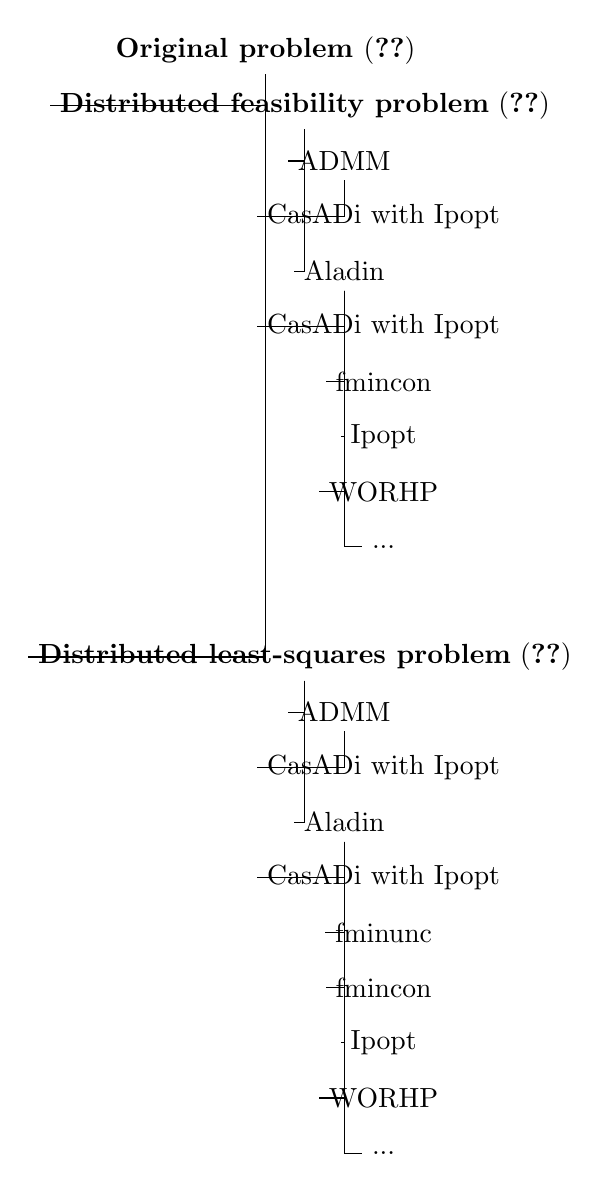
\begin{tikzpicture}[%
          grow via three points={one child at (0.5,-0.7) and
          two children at (0.5,-0.7) and (0.5,-1.4)},
          edge from parent path={(\tikzparentnode.south) |- (\tikzchildnode.west)}]
          \node {\textbf{Original problem~\eqref{eq:dist-power-flow-problem}}}
            child { node {\textbf{Distributed feasibility problem}~\eqref{eq:dist-feasibility-problem}}
                child { node{ADMM}
                    child { node{CasADi with Ipopt}}
                }
                child [missing] {}
                child { node{Aladin}
                    child { node{CasADi with Ipopt}}
                    child { node{fmincon}}
                    child { node{Ipopt}}
                    child { node{WORHP}}
                    child { node{...}}
                }
            }
            child [missing] {}
            child [missing] {}
            child [missing] {}
            child [missing] {}
            child [missing] {}
            child [missing] {}
            child [missing] {}
            child [missing] {}
            child [missing] {}	
            child { node {\textbf{Distributed least-squares problem}~\eqref{eq:dist-least-squares-problem}}
                child { node{ADMM}
                    child { node{CasADi with Ipopt}}
                }
                child [missing] {}
                child { node{Aladin}
                    child { node{CasADi with Ipopt}}
                    child { node{fminunc}}
                    child { node{fmincon}}
                    child { node{Ipopt}}
                    child { node{WORHP}}
                    child { node{...}}
                }
            };
        \end{tikzpicture}
        \caption{Algorithm Tree\label{fig: Algorithm-tree}}
    \end{figure}
\clearpage

\section{Graphical User Interface (GUI)}

To allow user interact with different algorithms and solvers in different problem formulation, a graphical user interface (GUI) is implemented, according the algorithm tree in \textbf{Figure~\ref{fig: Algorithm-tree}}. \textbf{Figure~\ref{fig:Graphical User Interface}} shows the GUI in morenet project.\\

Because the morenet project is on development, not all combinations listed are available. Check \textbf{\href{https://iai-vcs.iai.kit.edu/advancedcontrol/code/morenet/morenet/-/blob/Least_squares_problem/readme.md}{Readme.md}} for more details in current status.

\begin{figure}[hbt!]
 \begin{center}
    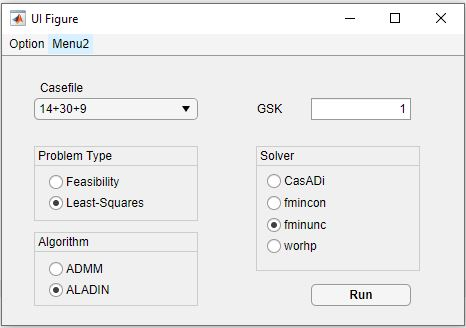
\includegraphics[width=0.8\textwidth]{visualization/GUI.JPG}
    \caption{:Graphical User Interface (GUI)}
    \label{fig:Graphical User Interface}
 \end{center}
\end{figure}
\clearpage
\newpage
\section{Simulation Result}

\subsection{Solve Feasibility Problem using ADMM}

\begin{itemize}
    \item Compare the results with different penalty parameter $\rho$
    
$\rho$ was set to $0.1$,$1$,$10$,$10^2$,$10^3$,$10^4$,$10^5$
. The upper in \textbf{Figure~\ref{fig:different penalty parameter}} shows the step-length to the optimum point and lower one shows the violations in norm-inf:
        \begin{figure}[hbt!]
         \begin{center}
            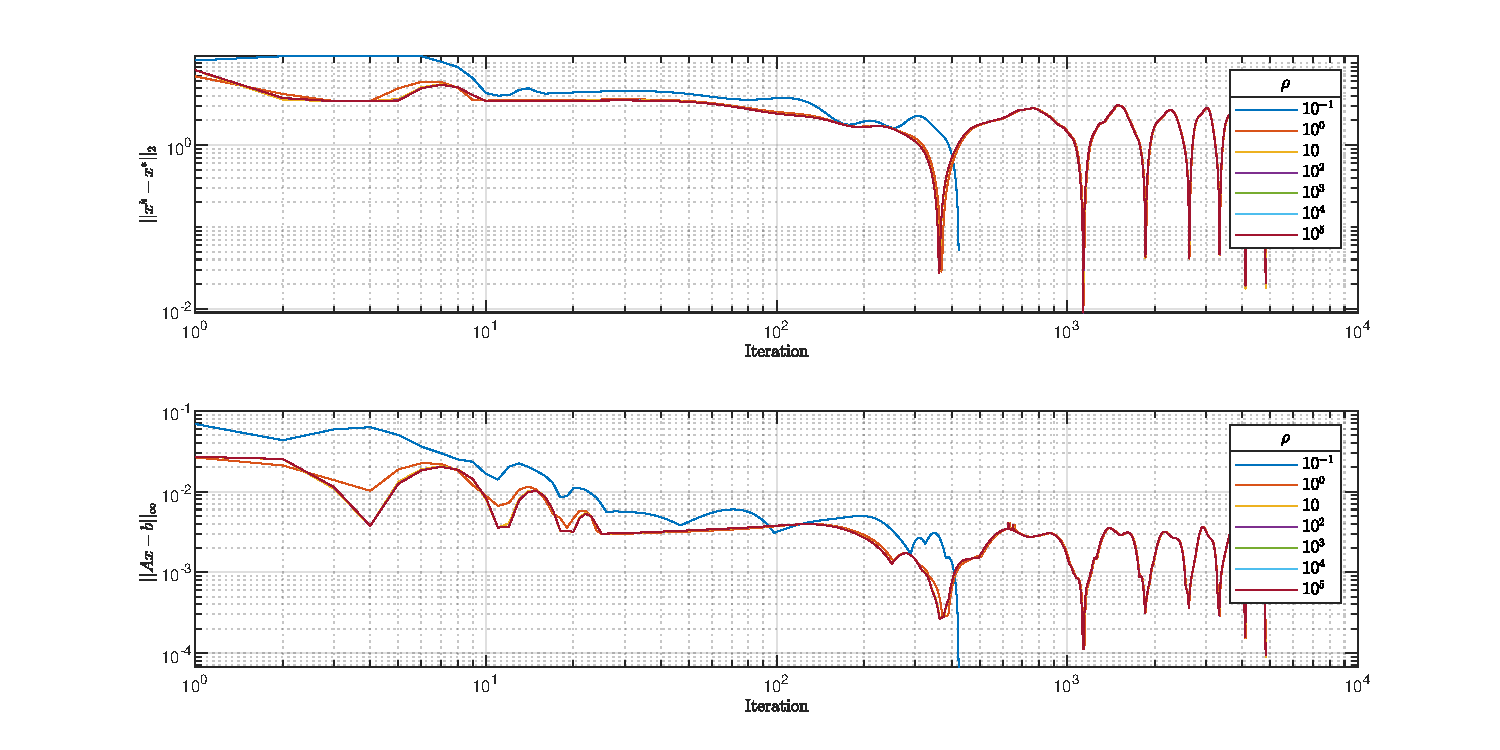
\includegraphics[width=1\textwidth]{Simulation_Results/comparision of different rho.pdf}
            \caption{Comparison of different penalty parameter $\rho$}
            \label{fig:different penalty parameter}
         \end{center}
        \end{figure}
         \begin{figure}[hbt!]
         \begin{center}
            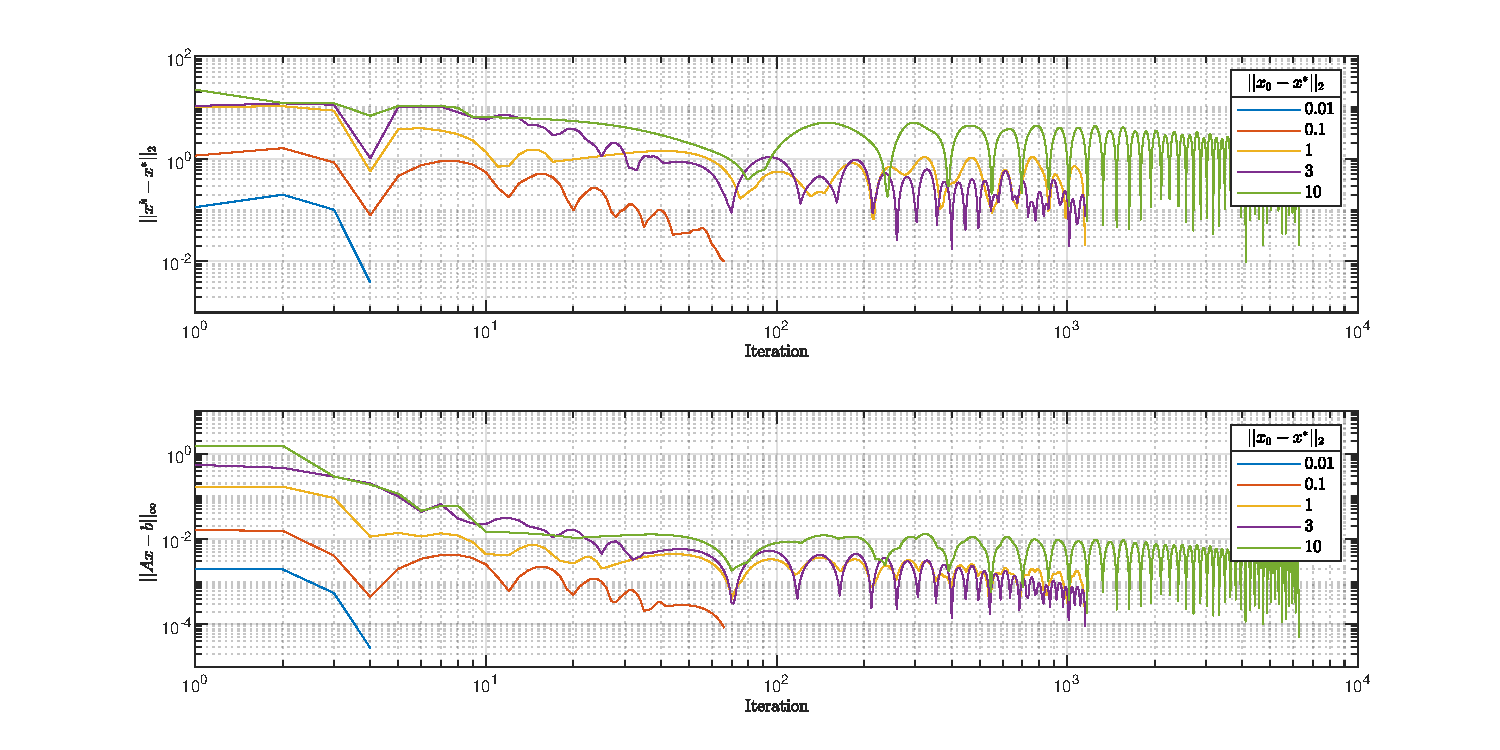
\includegraphics[width=1\textwidth]{Simulation_Results/comparision of different initial points.pdf}
            \caption{Comparison of different distance $\alpha$ between $x_0$ and $x^\ast$}
            \label{fig:different distance}
         \end{center}
        \end{figure}           

        
    \item Compare the results with different initial point


        Random initial points with fixed distance to the optimum,  $\alpha = \norm{x_0-x^\ast}$, were created in this task. The fixed distance $\alpha$ were set to $0.01,0.1,3,10$. Distance of each region was set to $\sqrt{\frac{\alpha}{N_{region}}}$, so that the distance of all state in norm-2 would be  $\alpha$
        
        The upper graphic in \textbf{Figure~\ref{fig:different distance}} shows the step-length to the optimum point and lower one shows the violations in norm-inf.
        

        
        The convergence rate depends on how far the initial point from the optimum is.\break
        

        
\end{itemize}
\noindent In Morenet cases, we face some trouble using ADMM to solve feasibility problem. Its performance depends on penalty parameter and it doesn't converge in most cases. Even it does converge, convergence rate is highly dependent from distance between optimum and initial point / initial guess. These increase challenges towards the realization in practice. \\

\noindent Hence, we stop investigating the feasibility problem with ADMM. Instead, we turns to ALADIN. In the following sections, problems are solved using ALADIN, which is proved to be very efficient in solving distributed non-convex  optimization problem.\\break
\newpage

\subsection{Solve Least-Squares Problem using ALADIN}

In earlier research, CasADi and fmincon are implemented to solve feasibility problem. However, it takes too long to run the algorithms, when the problem size goes from medium to large. To solve the problem withn a reasonable time, the problem type is transformed to least-squares problem. In \textbf{section~\ref{sec: comparison of solvers}}, several solvers are implemented in least-squares problem and their performance would be discuss. Later in \textbf{section~\ref{sec: comparison of solvers}}

\subsubsection{Comparison of different Solvers}~\label{sec: comparison of solvers}

\begin{enumerate}
\item CasADi \& IPOPT

In earlier research, CasADi \& IPOPT shows an ability to solve a small-to-medium size feasibility problems, namely the number of nodes is less than 300. With increasing number of nodes, setup time of a problem increase dramatically, while the duration of computing still remain  short in contrast. Thus we believe CasADi is the main bottleneck. However, IPOPT is still worth a try.

\item fmincon \& fminunc

\begin{figure}[hbt!]
 \begin{center}
    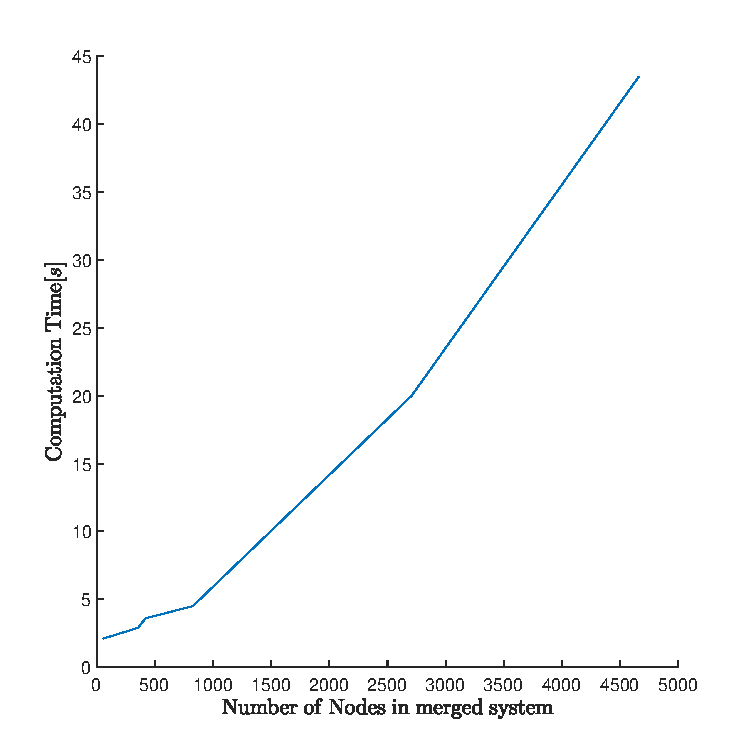
\includegraphics[width=0.6\textwidth]{Simulation_Results/Performance_of_fmincon.pdf}
    \caption{Performance of fmincon with Different Problem Size}
    \label{fig:performance of fmincon}
 \end{center}
\end{figure}

\textbf{Figure~\ref{fig:performance of fmincon}} shows computing time of fmincon, with different scale cases. Unlike CasADi, the computing time has a linear growth, even when the number of nodes near 5000. Also notice that sensitivities are computing according to \textbf{Section~\ref{sec: sensitivities computation}} with least-squres formulation. This means Gradient, Jacobian and Hessian are user-defined function-handle in fmincon solver.

\item WORHP

WORHP is designed to solve large-scale problem and input data should be transformed in a specific sparse form. First challenges of WORHP is how to feed the Hessian-information. It requires a special sorting of the sparse entries. All entries on the diagonal must be given, even structural zeros. Furthermore, the non-diagonal entries must be given first.~\cite{worhp} So the correct order of elements is supposed to be:
\begin{itemize}
  \item Nonzero elements in \textit{lower triangular matrix};
  \item All diagonal elements, including zero element.
\end{itemize}

In our model, sensitivities are saved in function-handle, a type of matlab data. After transformation, function-handle becomes complicated, and it would results in an error by WORHP. An intuitive solution is, instead of function-handle, hessian information is supported by a numerical matrix, when it is called by solver. Following code is an example of how it is done: 


\begin{minted}[mathescape,gobble=2]{csharp}
  /* wCallback   :         input struct for WORHP in matlab-interface
     build_Hess_vector():  the function to transform hessian matrix into vector  */
     
 wCallback.hm          = @(x)build_Hess_vector(Hess.Func(x)...);
\end{minted}

\item IPOPT

Installation of development environment for IPOPT in Windows OS is too complicated and the guides online are out-of-date. So we planned to implement it in Linux OS. Now, a Linux system, Ubuntu, has been created in VirtualBox and Maltab and WORHP has been installed. However, there are other prior tasks to do, this task still remain unfinished. 

\end{enumerate}

Simulation results of solving least-squares problem are showed in \textbf{Talbe~\ref{table: Computing Time Compared with Different Solver}}. By the problem with 418 nodes, system consists of a medium-size subsystem with 300 nodes. Meanwhile, the largest two problem, i.e. 2708 nodes and 4662 nodes, both include at least one large subsystem with more than 1000 nodes. It exhibited that size of subsystem has an critical influence of computation burden. \\
\begin{table}[hbt!]
\centering
 \begin{tabular}{||c c c c||}
 Number of Nodes & fminunc [s] & fmincon [s] & worhp [s]\\ [0.5ex] 
 \hline\hline
 53 & 2.5 & 2.2  & 2.4\\ 
 \hline
 354  & 2.5 & 3.1 & 4.8\\
 \hline
 418  & 4.5 & 5.2 & 7.0\\
 \hline
 826  & 3.7 & 5.3 & 7.2\\
 \hline
 1180  & 4.9 & 6.7 & 9.8 \\
 
 \hline
 2708  & 212.7 & 41.9 & 53.6\\ 
 \hline
 4662  &  387.9 & 90.1 & 113.8\\ [1ex] 
 \hline
\end{tabular}
\caption{Computing Time Compared with Different Solvers}
\label{table: Computing Time Compared with Different Solver}
\end{table}

In aspect of number of convergence rate, algorithm with all three different solver converges in the same iterations by a same problem. Compared with fmincon, fminunc is slightly faster. However, the computing time increases dramatically, when the local problem size is large. In general, fminunc is fastest solver for small-size problem, but is not able to handle large-scale problem.\\

On the contrary, fmincon and worhp are qualified even when the number of nodes increases to 1000+. During the simulation, it is observed that the setup-time of worhp is slower than fmincon. One of the reason could be that fmincon is a matlab-rooted solver, while worhp is coded in cpp and requires a worhp-matlab-interface to run in matlab. However, due to sparse form of data, worhp is supposed to have an ability to find minimum within a reasonable cost, when the problem size keep growing.

\begin{figure}[hbt!]
 \begin{center}
    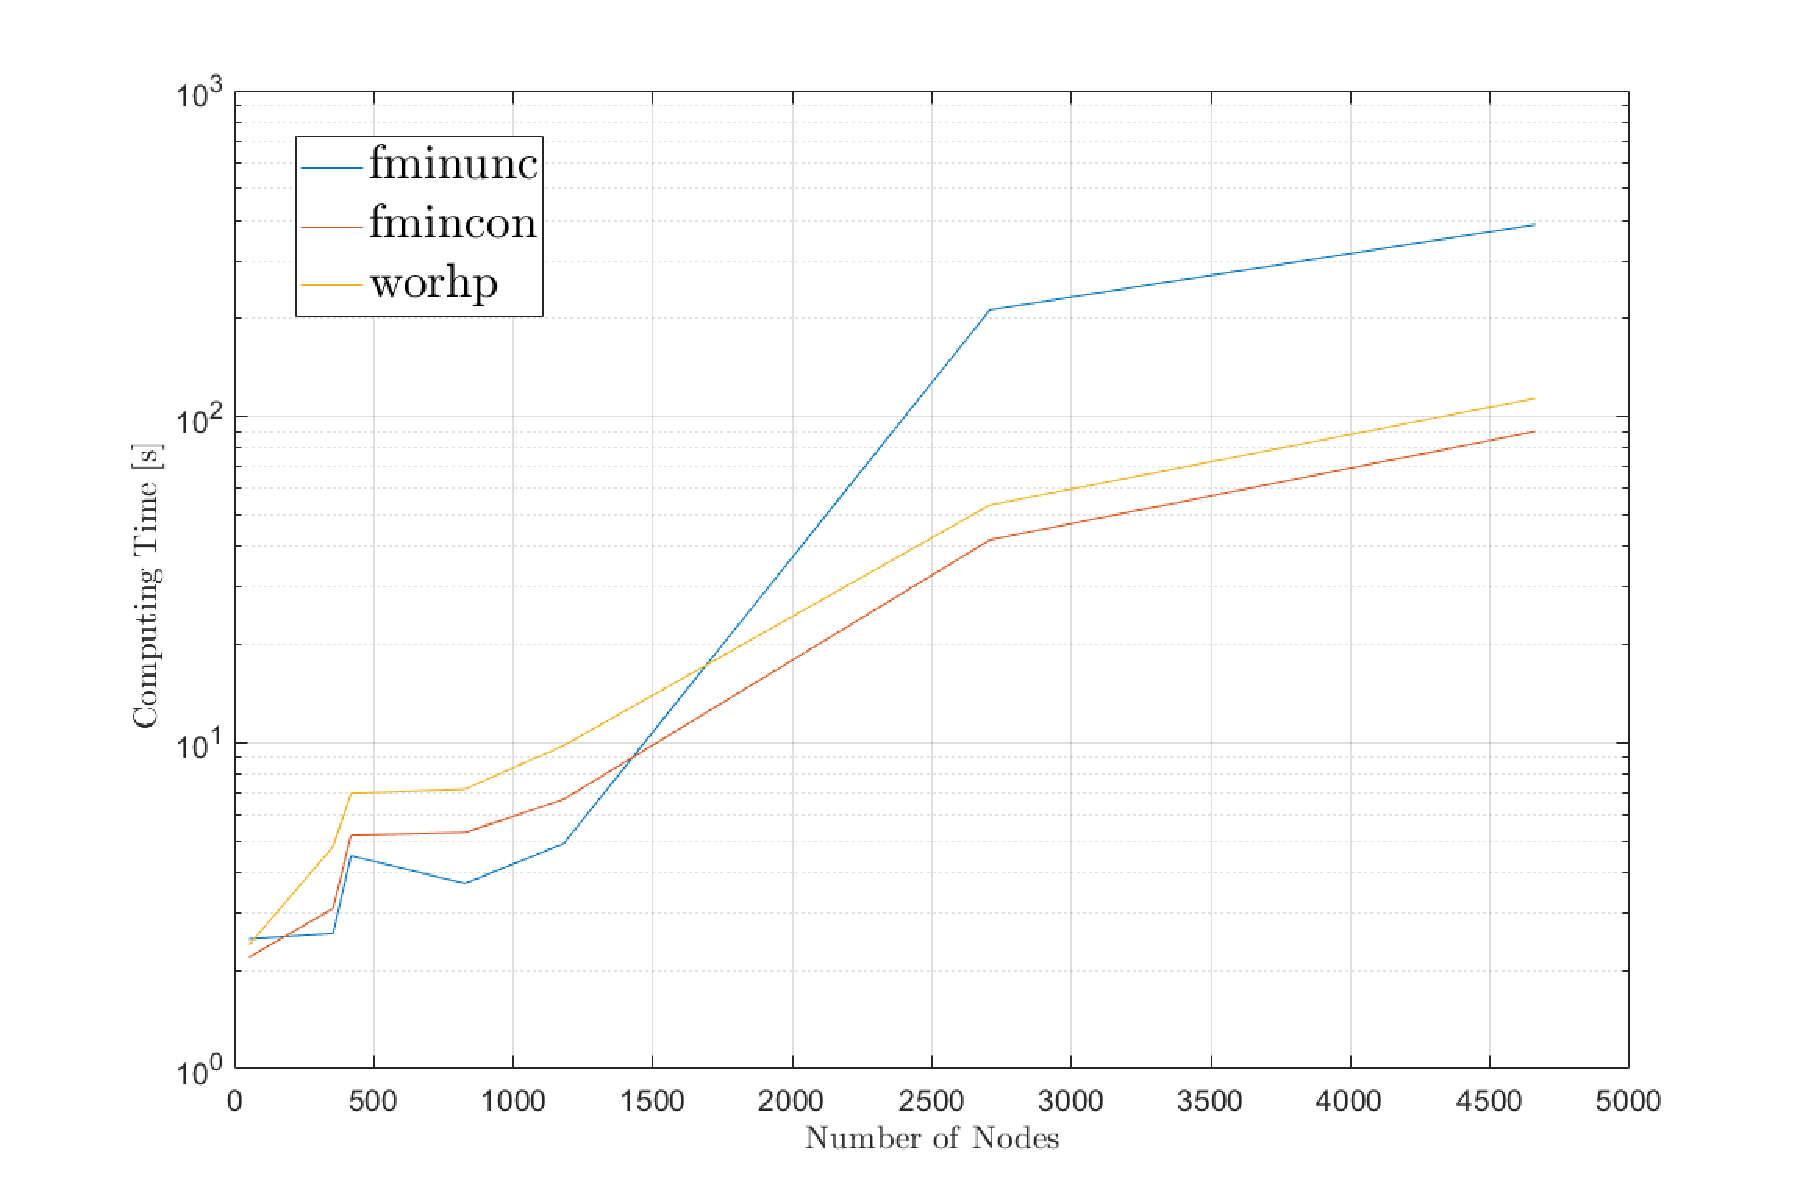
\includegraphics[width=1\textwidth]{Simulation_Results/computing_time_diff_solvers.pdf}
    \caption{computing time by different solvers}
    \label{fig:computing time by different solvers}
 \end{center}
\end{figure}
\clearpage

\subsubsection{Comparison of different Hessian Approximation Strategies}~\label{sec: different hessian approximations}

As described in \textbf{Section~\ref{sec: sensitivities computation}}, four methods are used to approximate Hessian, i.e. classic BFGS, limited-memory BFGS, Finite-Difference and approximation by Jacobian matrix $J_i(x_i)^T J_i(x_i)$ \\

As shown in \textbf{Table~\ref{table: Computing time compared with different Hessian approximations}} and \textbf{Figure~\ref{fig:computing time by different hessian approximations}}, approximation by Jacobian matrix has an amazing performance in all examples. In the meantime, the other three methods face convergence problem, when the problem size surpass 418 nodes. \\

Notice that, computing time of BFGS is intolerant, when the problem size of subsystem become medium (300 Nodes). 

\begin{table}[hbt!]
\centering
 \begin{tabular}{||c c c c c||}
 Number of Nodes & BFGS [s] & limit-memory BFGS [s] & Finite-difference [s] & user-defined [s]\\ [0.5ex] 
 \hline\hline
 53 & 28.6 & 22.9 & 10.0 & 2.2\\ 
 \hline
 354  & 287.8 & 107.4 & 61.5 & 3.1\\
 \hline
 418  & 1086.4 & 148.2 & 185.6 & 5.2\\  [1ex] 
\end{tabular}
\caption{Computing time compared with different Hessian approximations}
\label{table: Computing time compared with different Hessian approximations}
\end{table}
\begin{figure}[hbt!]
 \begin{center}
    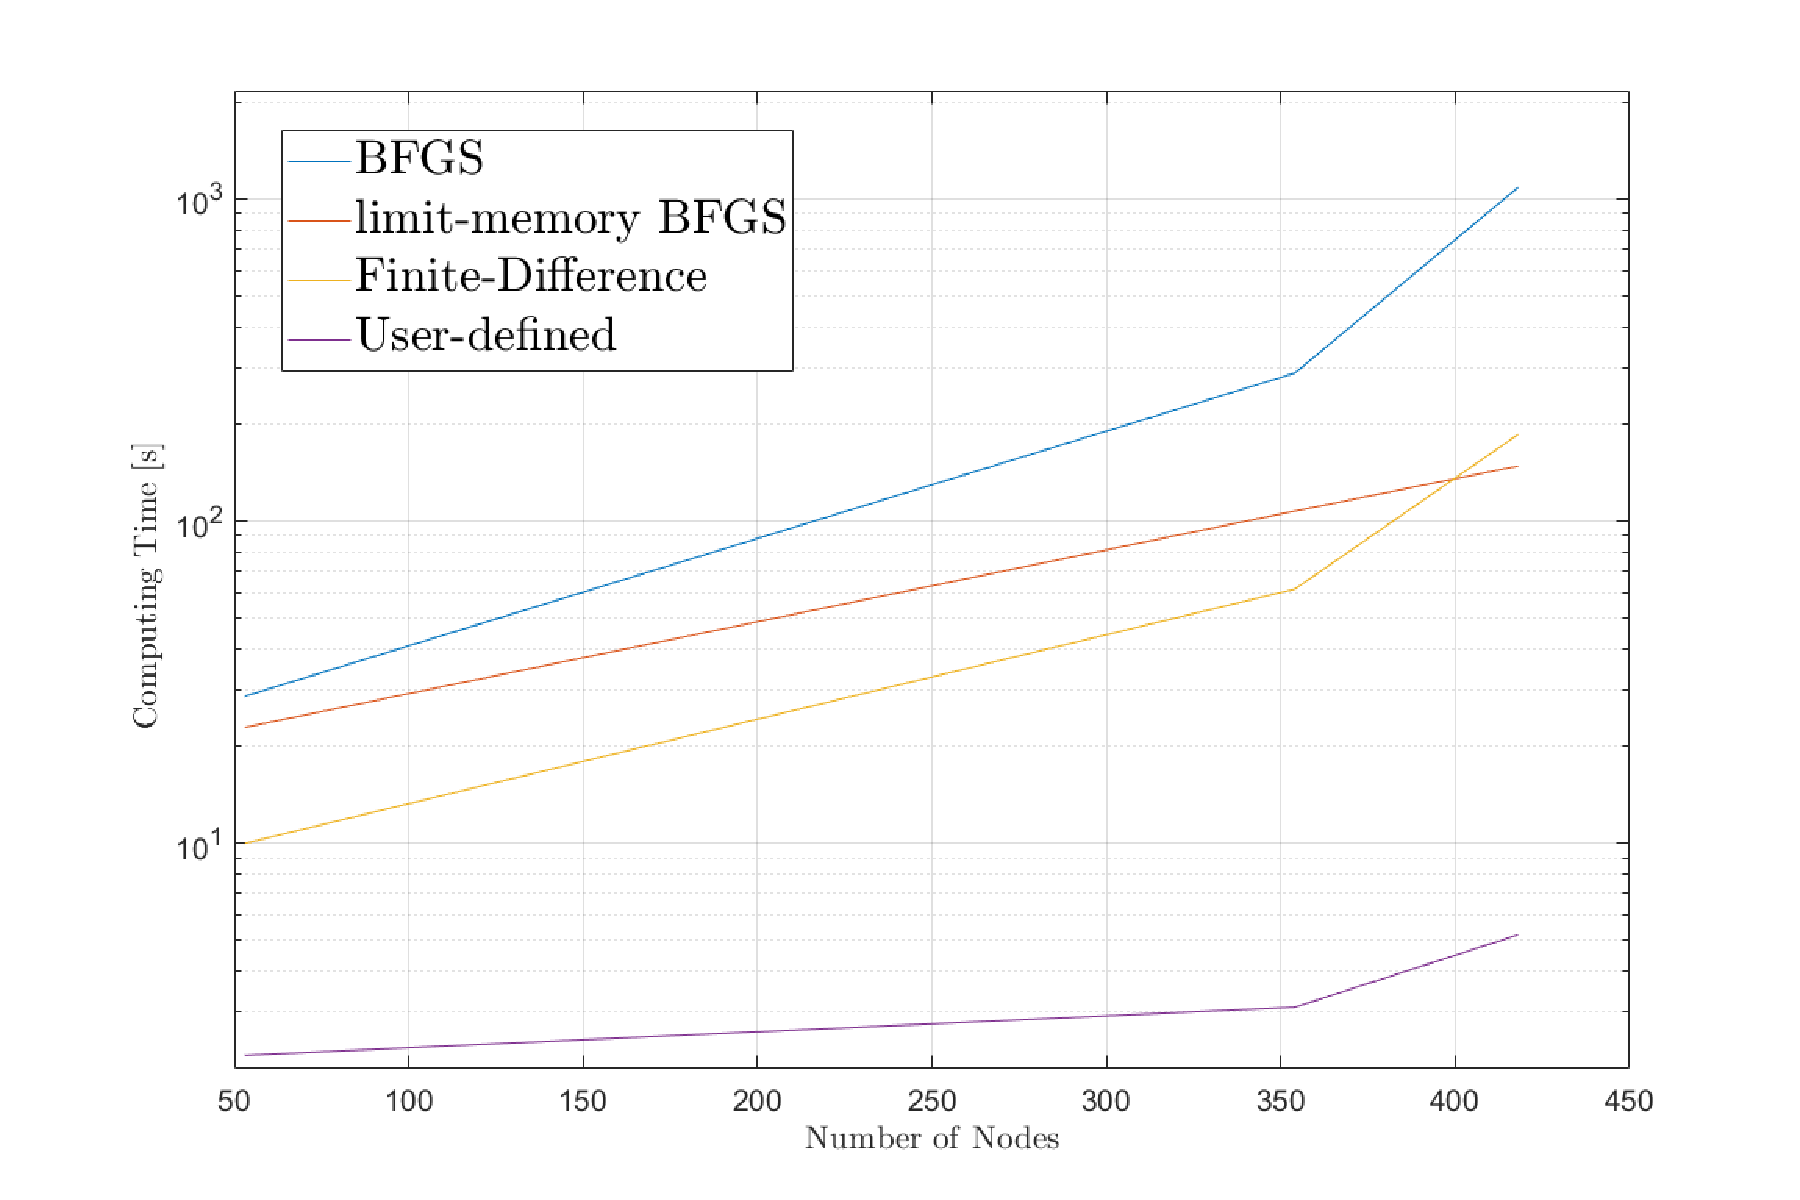
\includegraphics[width=1\textwidth]{Simulation_Results/computing_time_diff_hessian.pdf}
    \caption{computing time by different hessian approximations}
    \label{fig:computing time by different hessian approximations}
 \end{center}
\end{figure}

\newpage
\subsection{Generation Shift Key (GSK)}

In the example case, there are three region, i.e. 1, 2 and 3. Region 1 represents transmission system, while Region 2/3 represent two distribution systems. There are a transformer connected between Region 1 and Region 2. Meanwhile, there are two transformer connected between Region 2 and Region 3. \\

In each graphs in \textbf{Figure~\ref{fig:reduction of power}}, the first three bars represent a sum of generated real power in each region respectively, while 'i-j' bar represent the power flow between Region i and Region j. When the value is positive, power flow has the same direction as the arrow, vice versa.\\

\begin{figure}[hbt!]
\begin{subfigure}{.5\textwidth}
  \centering
  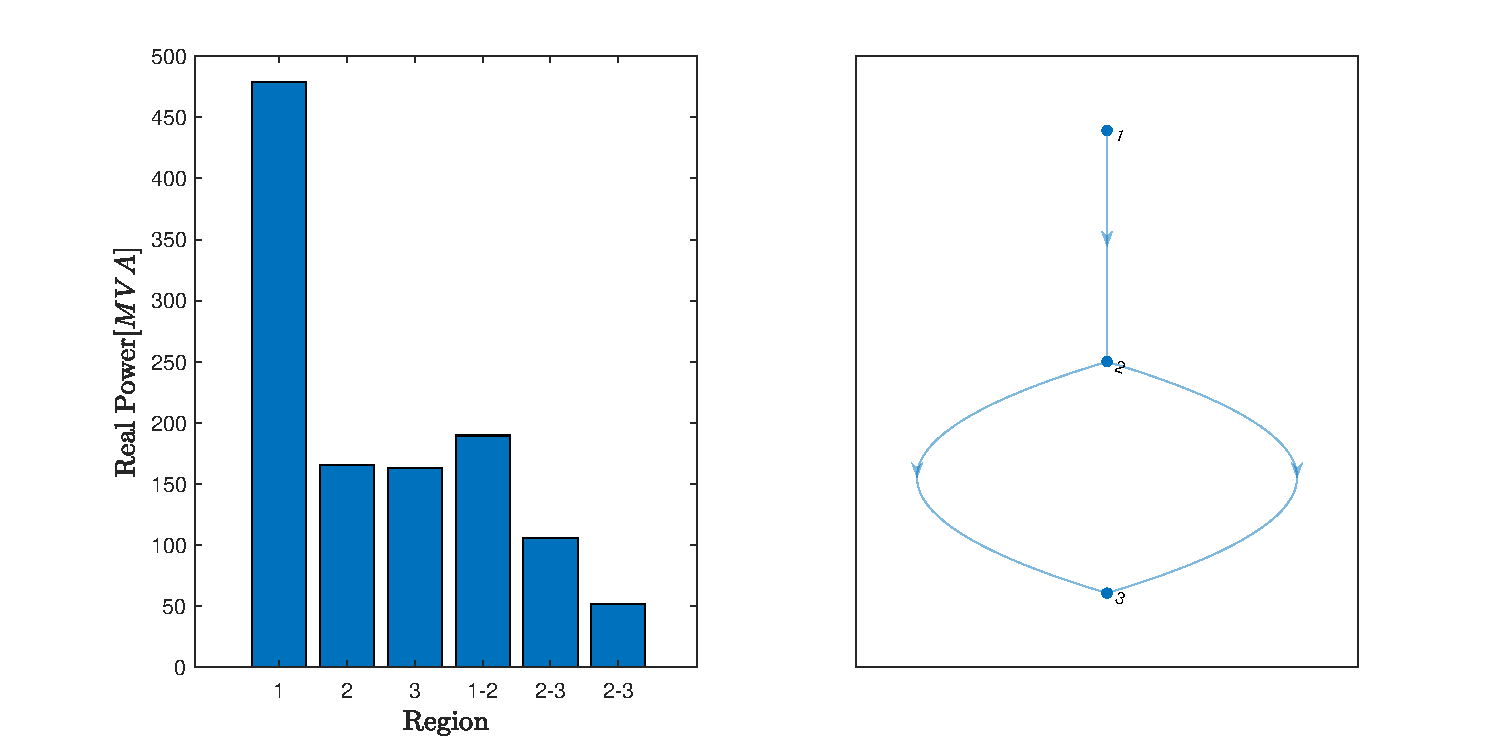
\includegraphics[width=0.9\linewidth]{Simulation_Results/unchanged.pdf}
  \caption{Remain unchanged}
  \label{fig:sfig1}
\end{subfigure}%
\begin{subfigure}{.5\textwidth}
  \centering
  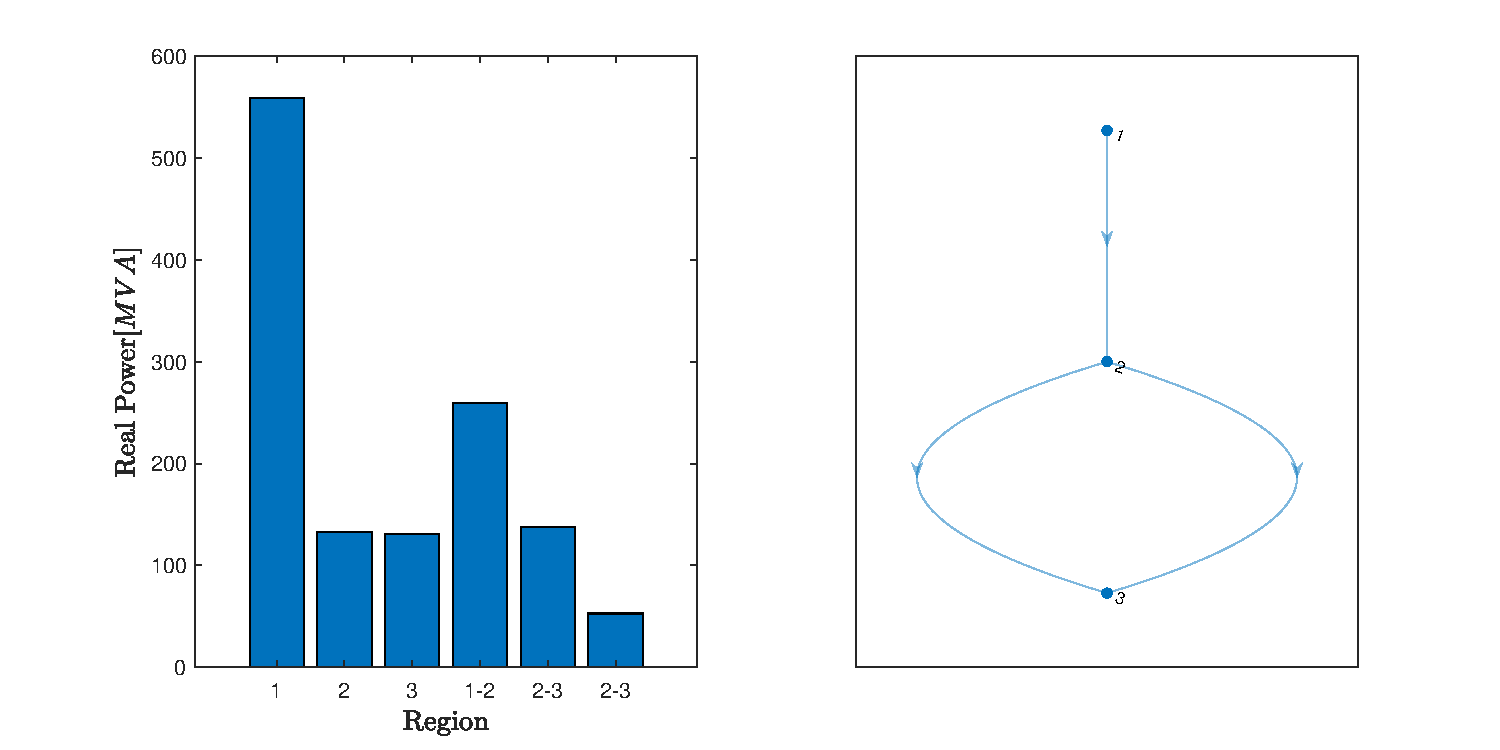
\includegraphics[width=0.9\linewidth]{Simulation_Results/reduce_to_80.pdf}
  \caption{Reduce to 80\%}
  \label{fig:sfig2}
\end{subfigure}
\begin{subfigure}{.5\textwidth}
  \centering
  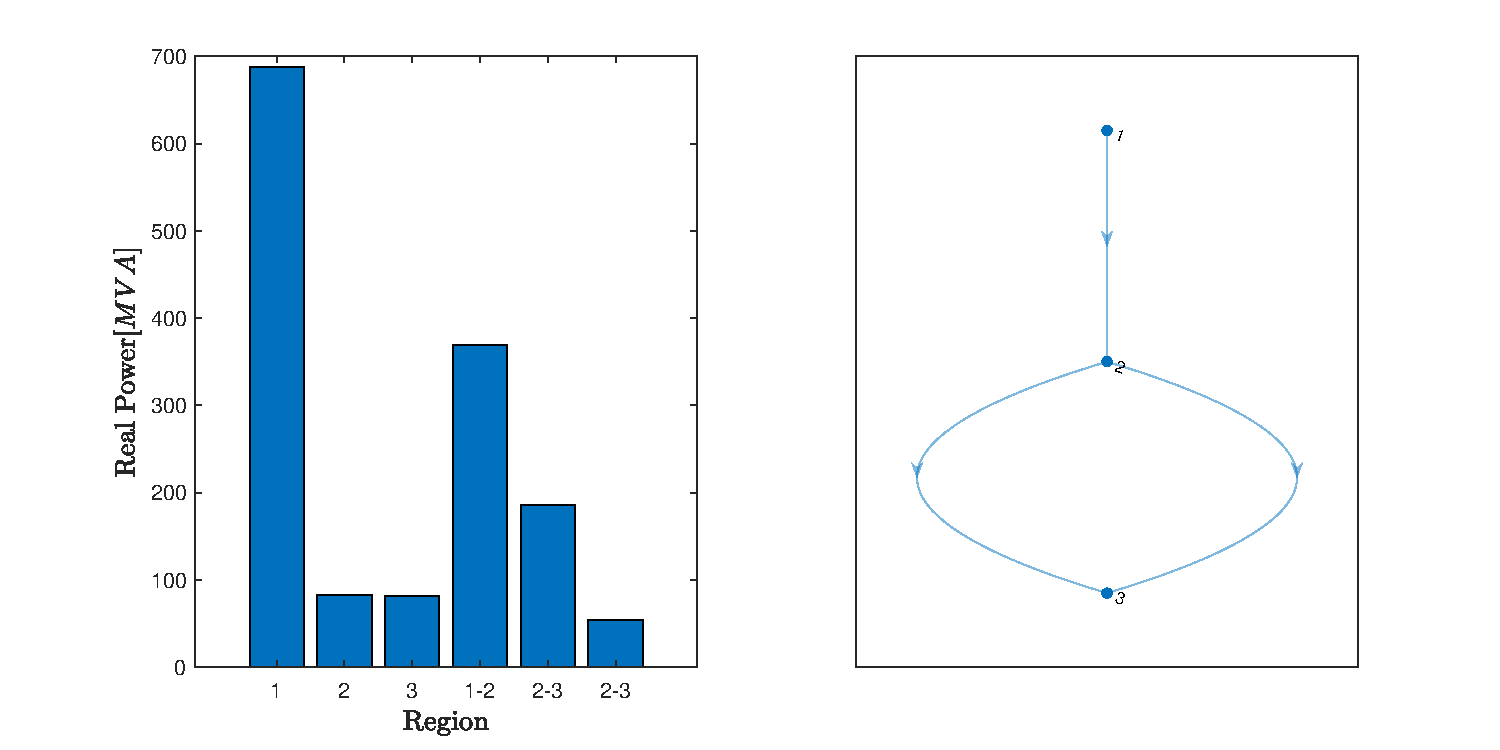
\includegraphics[width=0.9\linewidth]{Simulation_Results/reduce_to_50.pdf}
  \caption{Reduce to 50\%}
  \label{fig:sfig2}
\end{subfigure}
\begin{subfigure}{.5\textwidth}
  \centering
  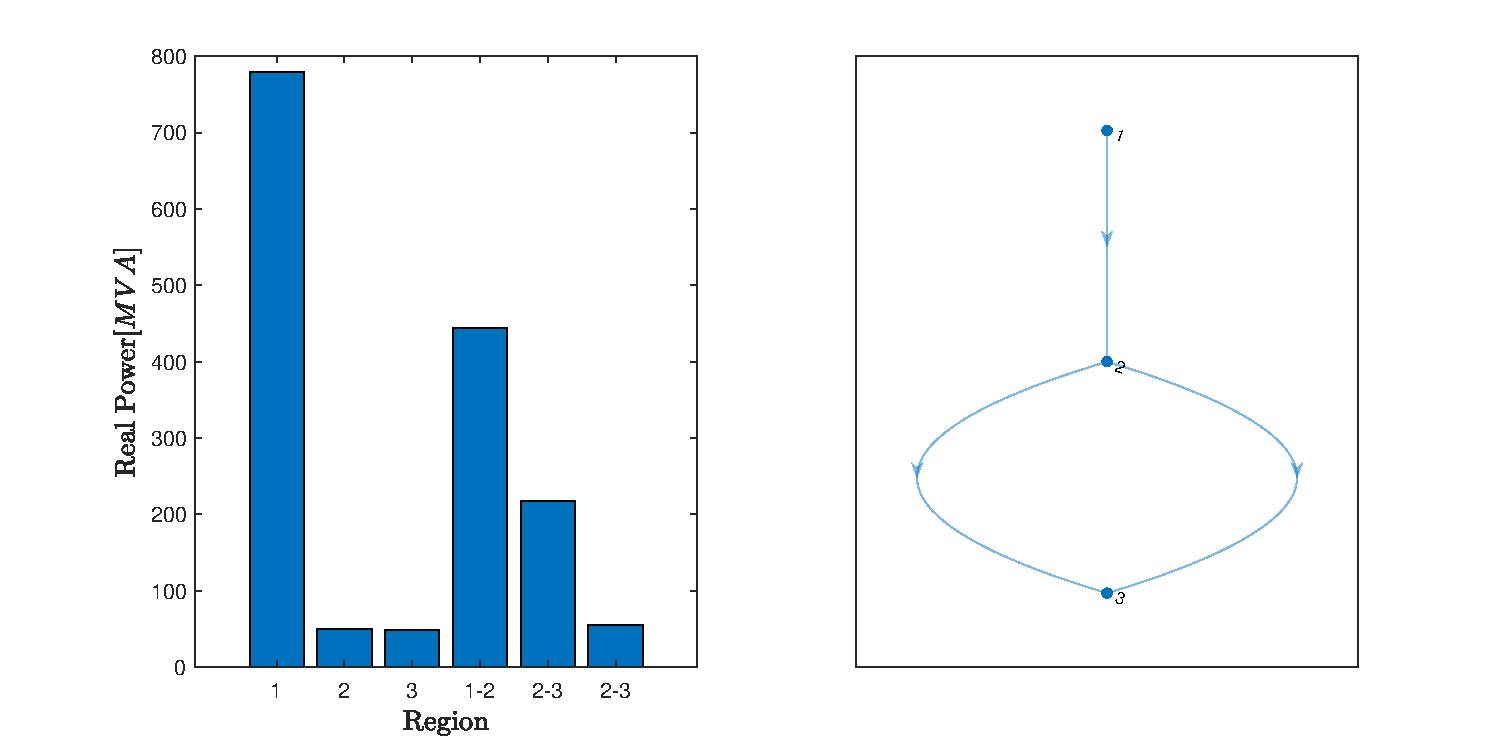
\includegraphics[width=0.9\linewidth]{Simulation_Results/reduce_to_30.pdf}
  \caption{Reduce to 30\%}
  \label{fig:sfig2}
\end{subfigure}
\caption{Reduction of Generated Power in Transmissions}
\label{fig:reduction of power}
\end{figure}

This new feature only works for small problem currently. For large-scale, i.e. number of nodes is more than $300$, reduction  will lead to infeasibility, when runpf() is called to validate the merged model. Even reduction to $90\%$ doesn't work. It is supposed that, although  reduction is small, the power flow between regions would increase dramatically because of larege number of nodes in total and violate constrains, e.g. line limit, which leads to infeasibility. 
\newpage
\section{Conclusion \& Future Work}

Although ADMM is proved to be not suitable for solving feasibility problem, investigating ADMM solving least-squares problem is still worthy, because the local cost function has been changed and there is no more equality constraints in local NLP step. \\

In aspect of Solver, approximating Hessian by $J_i(x_i)^T J_i(x_i)$ is a better solution, when the problem formulation changed to least-sqaures. On the one hand, it could decrease computation burden. On the other hand the approximation becomes more and more accurate, when $x$ approach minimum. However, for other forms of problem, computing or approximating Hessian is still a challenge, especially for a large-scale problem. In these case, limit-memory BFGS is worth trying. Another possible solution to large-scale problem, is to further partition the system, so that the local region size remains small.\\

Since Morenet project is based on matlab currently, fmincon, the matlab rooted funtion, is proved to be a more efficient solver and maintains a relative high performance for large-scale problem. However, this conclusion is highly platform dependent. If the project is planned to implement in practice, new research is needed to find out a suitable solver. \\

Meanwhile, there are still some tasks to be finished:\\

\begin{itemize}
    \item solve Least-sqaures problem by ADMM and compare with the results by ALADIN
    \item implement solver IPOPT in Linux OS
\end{itemize}

\bibliography{mybib}{}

\end{document}
